\documentclass{article}

% if you need to pass options to natbib, use, e.g.:
%     \PassOptionsToPackage{numbers, compress}{natbib}
% before loading neurips_2021

% ready for submission
\usepackage[preprint]{neurips_2021}

% to compile a preprint version, e.g., for submission to arXiv, add add the
% [preprint] option:
%     \usepackage[preprint]{neurips_2021}

% to compile a camera-ready version, add the [final] option, e.g.:
%     \usepackage[final]{neurips_2021}

% to avoid loading the natbib package, add option nonatbib:
% \usepackage[nonatbib]{neurips_2021}

\usepackage[utf8]{inputenc} % allow utf-8 input
\usepackage[T1]{fontenc}    % use 8-bit T1 fonts
\usepackage[colorlinks = true, 
		    linkcolor = blue,
		    urlcolor  = blue,
            citecolor = blue,
            anchorcolor = blue]{hyperref}       
% hyperlinks
\usepackage{url}            % simple URL typesetting
\usepackage{booktabs}       % professional-quality tables
\usepackage{amsfonts}       % blackboard math symbols
\usepackage{nicefrac}       % compact symbols for 1/2, etc.
\usepackage{microtype}      % microtypography
\usepackage{xcolor}         % colors
\usepackage{natbib}
\usepackage[pdftex]{graphicx}
\usepackage{siunitx} % Required for alignment
\sisetup{
  round-mode          = places, % Rounds numbers
  round-precision     = 2, % to 2 places
}
	
\bibliographystyle{unsrtnat}

% we did not really do a clustering
\title{Spotify metadata: Pop music is really less diverse}

% The \author macro works with any number of authors. There are two commands
% used to separate the names and addresses of multiple authors: \And and \AND.
%
% Using \And between authors leaves it to LaTeX to determine where to break the
% lines. Using \AND forces a line break at that point. So, if LaTeX puts 3 of 4
% authors names on the first line, and the last on the second line, try using
% \AND instead of \And before the third author name.

\author{%
  Dominik Glandorf\\
  Matrikelnummer 6007407\\
  \texttt{dominik.glandorf@student.uni-tuebingen.de} \\
  \And
  Felix D. Gross\\
  Matrikelnummer 6001480\\
  \texttt{fel.gross@student.uni-tuebingen.de} \\
}

\begin{document}

\maketitle

\begin{abstract}
% What did we do?
In this work we investigated if popular music is less diverse in terms of its variability.
% Why did we to it? What did we expect?
To assess the cliché contemporary pop music "being all the same",
% How did we do it?
metadata of 28,195 tracks on Spotify was collected, notably their popularity and audio features. To compare variability within popular versus non-pop songs, a Principal Component Analysis and F-tests were conducted.
% What did we find out?
A 2D-plot visually showed a difference between the groups. An analysis of variance confirmed that the diversity is indeed less in pop music, confirming our initial hypothesis.
% What now?
Conclusive, we discussed generalizability of our findings that is challenged by a potential sampling bias and imbalanced data.
\end{abstract}

\section{Introduction}
%Why are we interested in music?
Music is one of the oldest and most valued forms of communication and is therefore of particular interest. Yet, its underlying structure has been eluded systematic analysis until recently.
% What can we contribute?
Comparing numerous features across thousands of songs was too much data to handle with traditional tools of analysis. Accelerated computing and freely accessible databases allow now for systematic inquiry of a large music corpus. Thus, it is only now possible to hold common clichés about music proof to the real world data.
% What is our research question?
One of these clichés is, that pop music is all the same and less diverse then non-popular music \citep[see for example][]{serra2012measuring}. Thus, our hypothesis is, that the variability of pop music is smaller than the one inherent in non-popular music.

% What does music and popularity mean to us?
% TODO: add source for usage statistics and number of tracks
Since Spotify is the world's most used music streaming platform, it promises to be representative for global listening preferences. It additionally offers the largest corpus of music. For this reason, we rely on this single platform to define what is considered as music as well as what is considered as popular not only because such a big player has the data to set the bar for songs being popular but also enables us to quantify music due to its meta knowledge about tracks' properties.
% What is variability?
We define variability (and synonymously diversity) in the statistical sense of variance, i.e. the average squared distance from the mean. This variability is expected to be reflected in objective measures such as the tempo or subjective properties such as the danceability that Spotify is able to determine due to usage statistics and/or audio analysis.

\section{Method}

% TODO: add table here to list features:
% danceability, energy, liveness, loudness, speechiness, acousticness, instrumentalness, tempo, valence and key,
% Popularity: A value between 0 and 100 is assigned to each song, with 100 being the most popular.

\subsection{Sample}
% Where did we get the data exactly from?
The music metadata was obtained from the Spotify Web API \citep{spotifyAPIdocu}.
% How did exactly did we request our data?
In order to compile our sample, the search endpoint was queried in the following way: For each possible single Latin letter and two letter combination, the 50 first search results including their popularity score were stored. After eliminating duplicates in the result lists, the total sample encompassed \(N_{total} =\) 28,195 songs. The list of songs was then augmented by the results from the audio features endpoint.
% What are the columns/groups of our dataset?
The resulting features are explained in Table \ref{tab:features}. Songs with a popularity score of at least 90 were considered as pop songs. An inspection of the current charts and music played regularly in the radio led us to this admittedly arbitrary threshold. Based on it, the \(n_{pop} = 70\) most popular songs were assigned to the pop song group and the remainder \(n_{non pop} = 28,125\) to the non pop song group.

\begin{figure}
  \centering
  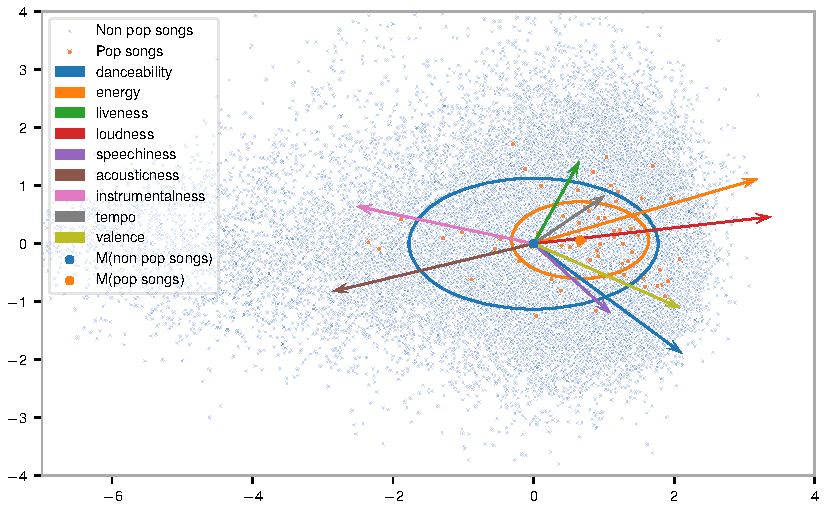
\includegraphics[]{../fig/001_pca.pdf}
  \caption{The projected sample on the first two principal components}
  \label{fig:pca}
\end{figure}

\subsection{Analysis}
% How did we ensure our data are appropriate?
To ensure data quality, we first graphically and numerically checked the distributions of our audio features and the popularity in the sample.

% How did we visually approached our hypothesis?
As stated above, we were interested in the variability of pop songs compared to the remainder. Hence, we first employed an exploratory and visual approach before running statistical tests. In order to search for an underlying structure in the audio features and to be able to get a first impression of the data as a whole we decided to do a dimensionality reduction via Principal Component Analysis (PCA). We decided against a stochastic neighbor embedding such as t-SNE since we only had 9 dimensions and believed in a global structure that might not be preserved by those methods. To be able to plot the principal components we chose the two components that explained the most variance. Since the PCA is agnostic to the grouping we indicated them in the visualization, in hope to see a structure.

% How did we statistically approached our hypothesis?
Independently of the results of the data exploration, we planned to conduct a two sample variance comparison on each audio feature \citep{snedecor1989}. Based on our hypothesis, that did not comprised mean differences in the two groups but rather variance differences, the weapon of choice was a classical F-test for independent samples. Because we conducted multiple F-tests we used the conservative instrument of the Bonferroni correction to decide for significance. To further assess our estimation quality we did a bootstrap sampling from both groups and calculated the variance quotient, i.e. the F-statistic for each of them. According to  here \cite{kruschke2014doing}
we calculated the 95\% HDI (highest density interval) that contains the 95\% of variance ratios that we most often encountered in the bootstrap procedure.

\section{Results}

\begin{figure}
  \centering
  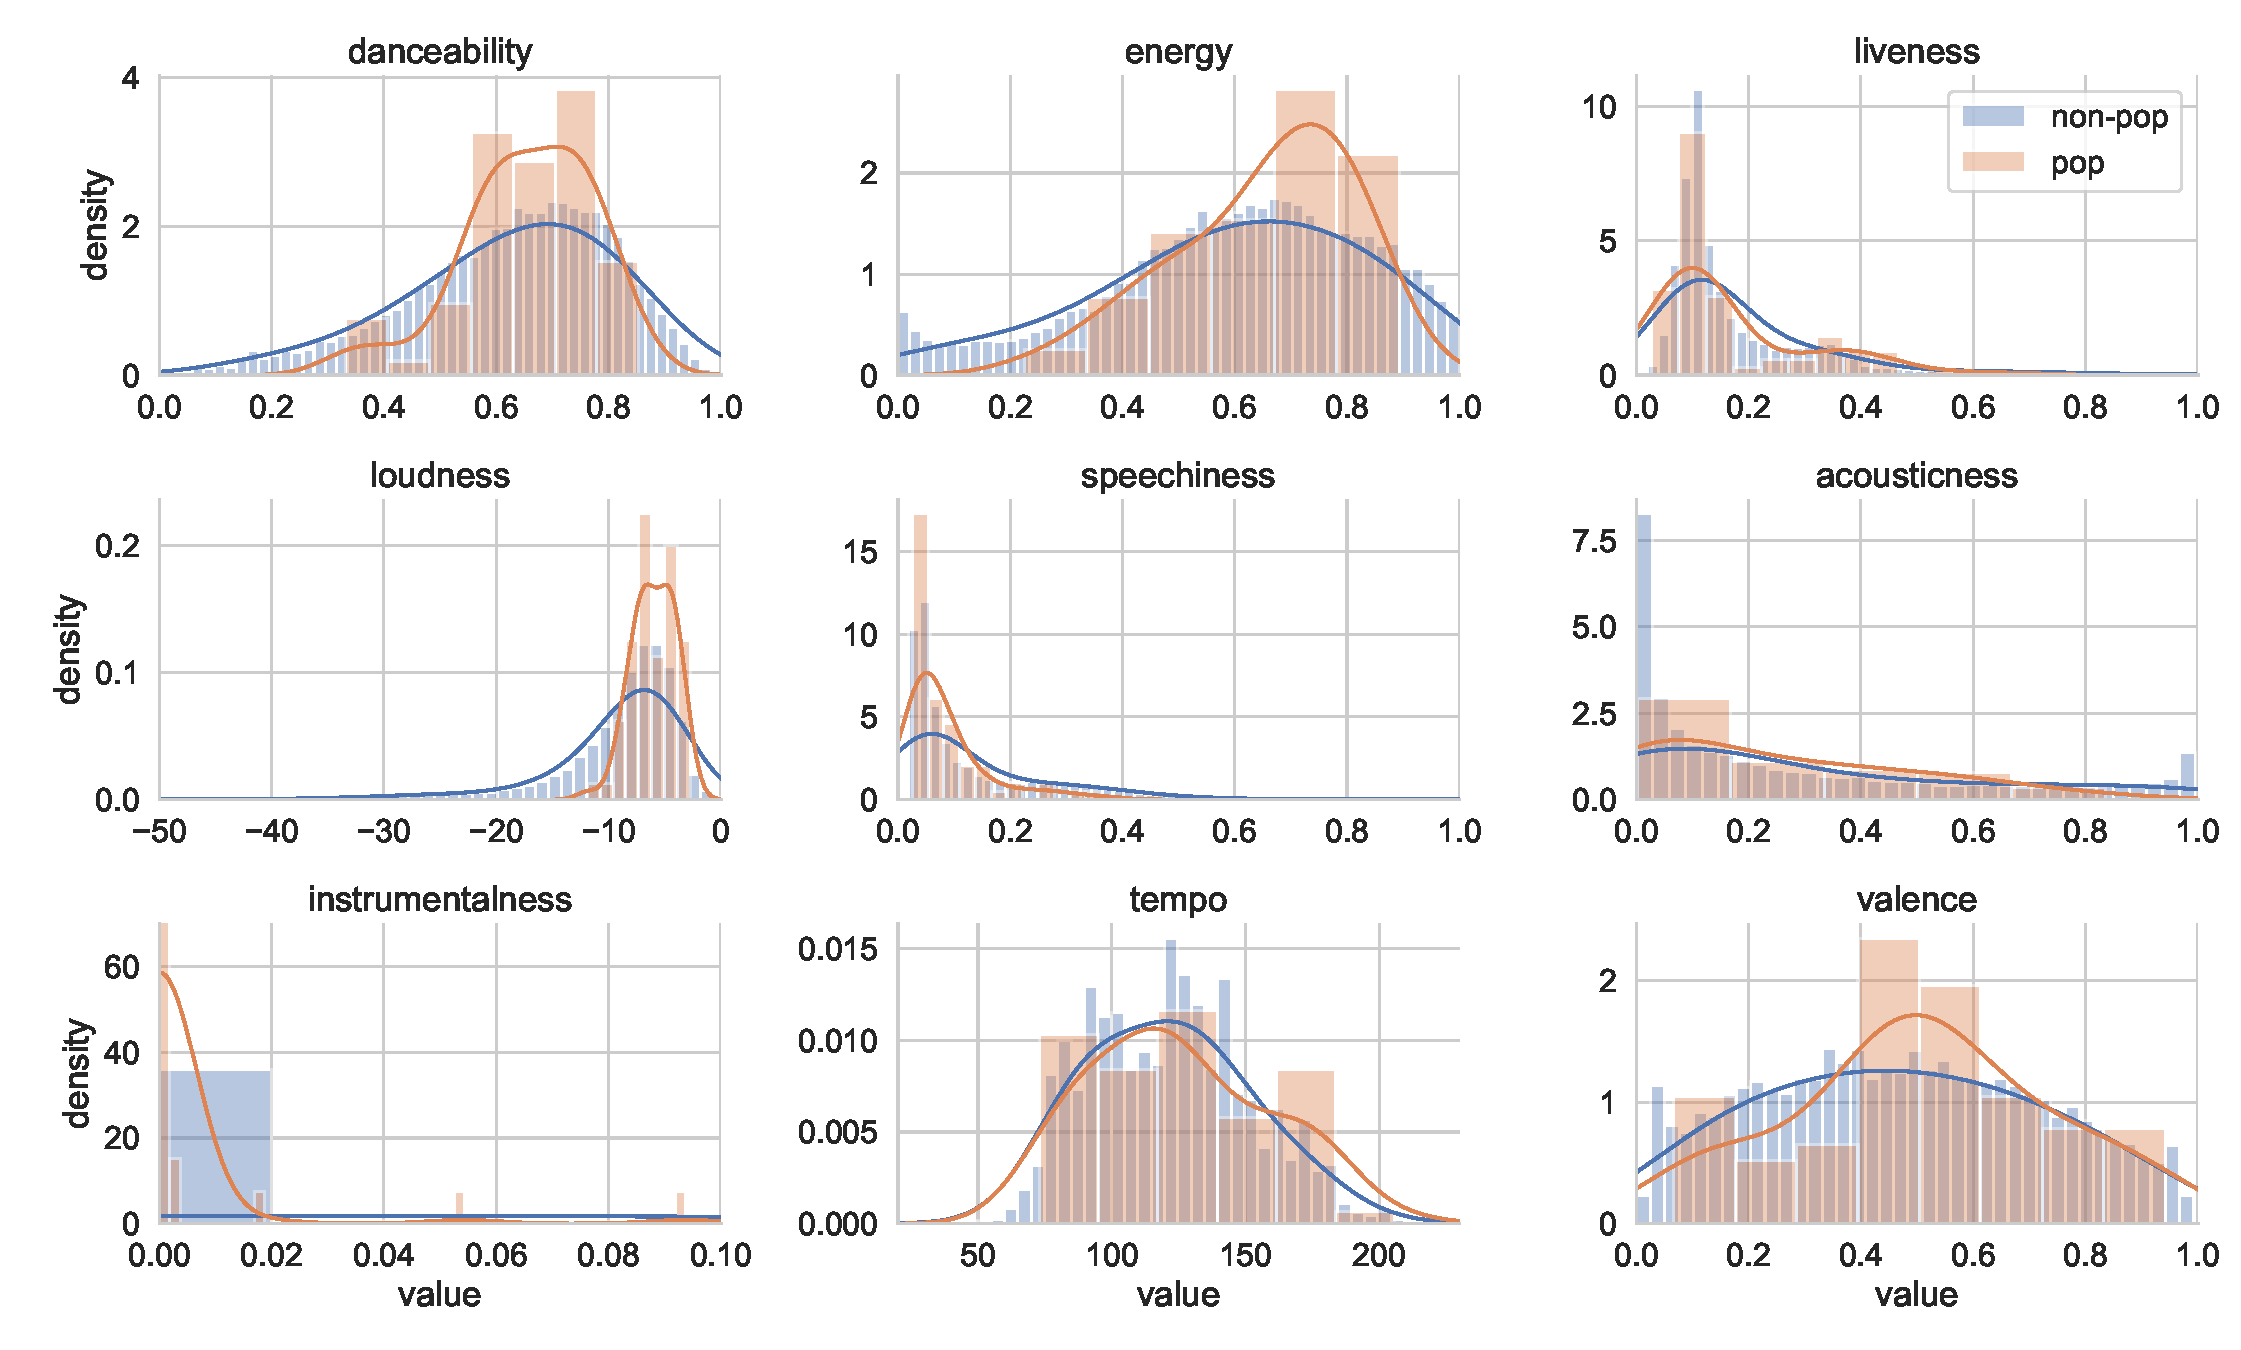
\includegraphics[width=1\linewidth]{../fig/002_variances.pdf}
  \vspace*{-15mm}
  \caption{Variances.}
\end{figure}

In Figure \ref{fig:pca} a 2D-visualization of the projected data points is shown. The popular songs clearly spread over an area contained in the bandwidth of the remaining songs. The standard variance within the first two principal components (PC) is visualized via the ellipses around the group means. This underlines the visual impression of lower variance of the popular songs. The mean of them is positively shifted mainly on the first PC. To understand how the original features load onto the PCs their loadings are indicated in an arbitrary scale via the arrows originating from the data's origin. The first PC is mainly determined by loudness and energy (positive loading) as well as instrumentalness and acousticness (negative loading). This PC could be seen as the "pop" dimension since today's popular songs are generally known to be energetic and well-produced (which results in a higher loudness feature) and less instrumental or acoustic (since those are perceived as stripped versions of the original music). The second PC shows the same pattern of less variance in the pop songs, even though it is less prominent. It is mainly based on liveness, speechiness, valence, danceability and tempo. Due to the very small mean difference those features seem to be not different in popular songs yet less variant. From the dimensionality reduction we can conclude that popular music seems to be actually less diverse in terms of its audio features and is also different on average.

\begin{table}[h!]
  \caption{Variance test results}
  \label{tab:var}
  \centering
  \begin{tabular}{lllc}
    \toprule
    Feature     & F-value & 95\% HDI\\
    \midrule
	danceability        	&  2.50** &\\
	energy              		&  2.26** &\\
	liveness            		&  1.23   &\\
	loudness            	&  9.27** &\\
	speechiness         	&  3.57** &\\
	acousticness        	&  1.80*  &\\
	instrumentalness    	&642.00** &\\
	tempo               		&  0.83   &\\
	valence             	&  1.21   &\\
    \bottomrule
  \end{tabular}
\end{table}


% no real correlation
% non-normal distribution of some features

% Variance tests results
Six of the tested features  % which audio features are significant?

\section{Discussion}
The variance of six of the evaluated nine features was significantly less in the pop-music group, if compared to the non-pop music group, hereby supporting our hypothesis of pop music being all the same.  
The unusual high variance difference 
Mixfeatures


nine features between 

% is our sampling strategy adequate?
% are we okay with the blackbox calculation of our features?

% imbalanced data, justify why it is inherent in our analysis and why we think that our results are still not biased by this imbalance
 It resulted  to be a suitable size for a hit parade, most of Spotify's own hit play-lists consist out of 50 songs, 
-other features
-other pop treshold (continous descibtion)

% Future research ideas:
% consider different markets/cultures, Spotify is heavily based to Western music, suggestion for further research, replicate our analysis for each countries charts

% Check over time, if there is a change or manifestation in variance ratios.

% Look at the output and repair capitalization and 
\bibliography{library.bib}

\end{document}
